\subsection{Scheme of an OR study}

The most important and common \textbf{steps} in operational research are:
\begin{enumerate}
    \item \textbf{Problem}. Define the problem;
    \item \textbf{Model}. Build the model;
    \item \textbf{Algorithm}. Select or develop an appropriate algorithm;
    \item \textbf{Implementation}. Implementing or using an efficient computer program;
    \item \textbf{Results}. Analyze the results.
\end{enumerate}

\begin{definitionbox}
    A mathematical \definitionWithSpecificIndex{model}{Model} is a \textbf{simplified representation of a real-world problem}.
\end{definitionbox}

\noindent
To define a mathematical model, it is necessary to identify the fundamental elements of the problem and the main relationships between them. But \textbf{how can we decide} the \emph{number of decision makers}, the \emph{number of objectives} and the \emph{level of uncertainty in the parameters}? It depends on the environment. If we have:
\begin{itemize}
    \item One decision maker, one object, then we will use \textbf{mathematical programming} (section \ref{subsection: Mathematical programming/optimization}, page \pageref{subsection: Mathematical programming/optimization}).
    \item One decision maker, multiple objectives, then we will use \textbf{multi-objective programming} (section \ref{subsection: Multi-objective programming}, page \pageref{subsection: Multi-objective programming}).
    \item Uncertainty greater than zero, then we will use \textbf{stochastic programming}.
    \item Multiple decision makers, then we will use \textbf{game theory}.
\end{itemize}

\highspace
\begin{examplebox}[: production planning]
    A company produces 3 types of electronic devices: $D_{1}$, $D_{2}$, $D_{3}$; going through 3 main phases of the production process: assembly, refinement and quality control.

    Time (in minutes) required for each phase and product:

    \begin{center}
        \begin{tabular}{@{} c | c c c @{}}
            & $D_{1}$ & $D_{2}$ & $D_{3}$ \\
            \midrule
            Assembly        & $80$ & $70$ & $120$ \\
            Refinement      & $70$ & $90$ & $20$ \\
            Quality control & $40$ & $30$ & $20$
        \end{tabular}
    \end{center}

    Available resources within the planning horizon (depend on the workforce) in minutes:
    \begin{center}
        \begin{tabular}{@{} c | c | c @{}}
            Assembly & Refinement & Quality control \\
            \midrule
            $30'000$ & $25'000$ & $18'000$
        \end{tabular}
    \end{center}

    Unitary profit (in KEuro):
    \begin{center}
        \begin{tabular}{@{} c | c | c @{}}
            $D_{1}$ & $D_{2}$ & $D_{3}$ \\
            \midrule
            $1.6$ & $1$ & $2$
        \end{tabular}
    \end{center}
    
    Assumption: the company can sell whatever it produces.

    \emph{Give a mathematical model for determining a production plan which maximizes the total profit.}

    \begin{itemize}
        \item \textbf{Decision variables}, $x_{j}$ is equal to the number of devices $D_{j}$ produced, for $j = 1, 2, 3$.
        
        \item \textbf{Objective function}: $\max \: z = 1.6x_{1} + 1x_{2} + 2x_{3}$.

        \item \textbf{Constraints}: the production capacity limit for each phase:
        \begin{equation*}
            \begin{array}{rcl}
                80x_{1} + 70x_{2} + 120x_{3} &\le& 30'000 \hspace{2em} \text{(assembly)} \\ [.5em]
                70x_{1} + 90x_{2} + 20x_{3} &\le& 25'000 \hspace{2em} \text{(refinement)} \\ [.5em]
                40x_{1} + 30x_{2} + 20x_{3} &\le& 18'000 \hspace{2em} \text{(quality control)}
            \end{array}
        \end{equation*}

        \item \textbf{Non-negative variables}: $x_{1}, x_{2}, x_{3} \ge 0$ may be fractional (real) values.
    \end{itemize}
\end{examplebox}

\begin{examplebox}[: portfolio selection problem]
    An insurance company must decide which investments to select out of a given set of possible assets (stocks, bonds, options, gold certificates, real estate, \dots).

    \begin{center}
        \begin{tabular}{@{} c | c c c @{}}
            Investments & area & capital $\left(c_{j} \: K\text{\euro}\right)$ & expected return $\left(r_{j}\right)$ \\
            \midrule
            A & Germany & $150$ & $11\%$ \\
            B & Italy & $150$ & $9\%$ \\
            C & U.S.A. & $60$ & $13\%$ \\
            D & Italy & $100$ & $10\%$ \\
            E & Italy & $125$ & $8\%$ \\
            F & France & $100$ & $7\%$ \\
            G & Italy & $50$ & $3\%$ \\
            H & UK & $80$ & $5\%$
        \end{tabular}
    \end{center}
    Legend:
    \begin{itemize}
        \item A and B: automotive
        \item C and D: ICT
        \item E and F: real estate
        \item G: short term treasury bounds
        \item H: long term treasury bounds
    \end{itemize}
    The available capital is: $600$ KEuro.

    At most 5 investments to avoid excessive fragmentation.

    Geographic diversification to limit risk: $\le 3$ investments in Italy and $\le 3$ abroad.

    \emph{Give a mathematical model for deciding which investments to select so as to maximize the expected return while satisfying the constraints.}

    \begin{itemize}
        \item \textbf{Decision variables}, $x_{j}$ is equal to $1$ if $j$-th investment is selected and $x_{j}=0$ otherwise, for $j = 1, \dots, 8$.
        
        \item \textbf{Objective function}: $\max \: z = \displaystyle\sum_{j=1}^{8} c_{j} \: r_{j} \: x_{j}$.

        \item \textbf{Constraints}:
        \begin{equation*}
            \begin{array}{rclcl}
                \displaystyle\sum_{j=1}^{8}c_{j} \: x_{j} &\le& 600 &\hspace{1em}& \text{(capital)} \\ [2em]
                \displaystyle\sum_{j=1}^{8}x_{j} &\le& 5 &\hspace{1em}& \text{(max 5 investments)} \\ [2em]
                x_{2}+x_{4}+x_{5}+x_{7} &\le& 3 &\hspace{1em}& \text{(max 3 in Italy)} \\ [.5em]
                x_{1}+x_{3}+x_{6}+x_{8} &\le& 3 &\hspace{1em}& \text{(max 3 abroad)}
            \end{array}
        \end{equation*}

        \item \textbf{Binary (integer) variables}: $x_{j} \in \left\{0,1\right\}$ and $1 \le j \le 8$.
    \end{itemize}

    \underline{\textbf{Possible variant}}. In order to limit the risk, if any of the ICT investment is selected then at least one of the treasury bond must be selected.
    \begin{itemize}
        \item \textbf{Objective function}: $\max z = \displaystyle\sum_{j=1}^{8} c_{j} \: r_{j} \: x_{j}$.

        \item \textbf{Constraints}:
        \begin{equation*}
            \begin{array}{rcll}
                \displaystyle\sum_{j=1}^{8}c_{j} \: x_{j} &\le& 600 & \text{(capital)} \\ [2em]
                \displaystyle\sum_{j=1}^{8}x_{j} &\le& 5 & \text{(max 5 investments)} \\ [2em]
                x_{2}+x_{4}+x_{5}+x_{7} &\le& 3 & \text{(max 3 in Italy)} \\ [.5em]
                x_{1}+x_{3}+x_{6}+x_{8} &\le& 3 & \text{(max 3 abroad)} \\ [1em]
                \dfrac{x_{3} + x_{4}}{2} &\le& x_{7} + x_{8} & \text{(investment in treasury bonds)}
            \end{array}
        \end{equation*}

        \item \textbf{Binary (integer) variables}: $x_{j} \in \left\{0,1\right\}$ and $1 \le j \le 8$.
    \end{itemize}
\end{examplebox}

\newpage

\begin{examplebox}[: facility location]
    Consider 3 oil pits, located in positions $A$, $B$ and $C$, from which oil is extracted.

    \begin{center}
        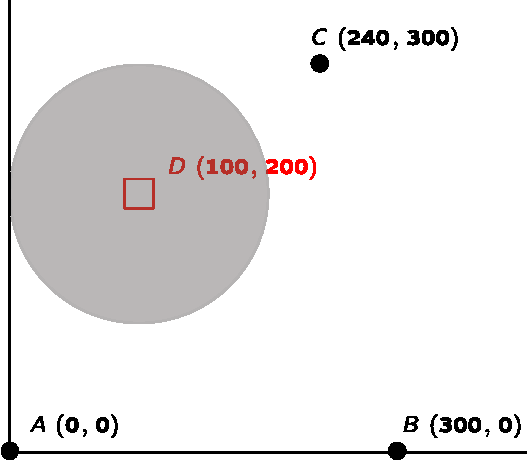
\includegraphics[width=.6\textwidth]{img/facility-location-1.pdf}
    \end{center}

    Connect them to a refinery with pipelines whose cost is proportional to the square of their length.

    The refinery must be at least 100 km away from point $D = \left(100, 200\right)$, but the oil pipelines can cross the corresponding forbidden zone.

    \emph{Give a mathematical model to decide where to locate the refinery so as to minimize the total pipeline cost.}

    \begin{itemize}
        \item \textbf{Decision variables}, $x_{1}, x_{2}$ cartesian coordinates of the refinery.
        
        \item \textbf{Objective function}:
        \begin{equation*}
            \begin{array}{rl}
                \min z = & \left[\left(x_{1} - 0\right)^{2} + \left(x_{2} - 0\right)^{2}\right] + \\ [.5em]
                         & \left[\left(x_{1} - 300\right)^{2} + \left(x_{2} - 0\right)^{2}\right] + \\ [.5em]
                         & \left[\left(x_{1} - 240\right)^{2} + \left(x_{2} - 300\right)^{2}\right]
            \end{array}
        \end{equation*}

        \item \textbf{Constraints}:
        \begin{equation*}
            \sqrt{
                \left(x_{1}-100\right)^{2} + \left(x_{2} - 200\right)^{2}
            } \ge 100
        \end{equation*}

        \item \textbf{Variables}: $x_{1}, x_{2} \in \mathbb{R}$.
    \end{itemize}
\end{examplebox}